\documentclass[12pt,letterpaper]{article}
\usepackage[utf8]{inputenc}
\usepackage[english]{babel}
\usepackage{ragged2e}
\usepackage[colorlinks = true,
            linkcolor = purple,
            urlcolor  = blue,
            citecolor = blue,
            anchorcolor = blue]{hyperref}
\hypersetup{
    colorlinks=true,
    linkcolor=blue,
    filecolor=blue,      
    urlcolor=blue,} 
\urlstyle{same}


\usepackage{ifpdf}
\usepackage{mla}

\begin{document}

\begin{mla}{Michael}{Brodskiy}{Mrs. Greer}{AP Language}{October 8, 2020}{\underline{Analyzing Political Cartoons}} 

  \begin{justifying}

    \paragraph{I.} In S.J. Ray and K.C. Star's cartoon entitled, ``The Rude Awakening,'' Ray and Star depict Adolf Hitler's dazed and perturbed state, with respect to the Eastern Front, through the use of a hyperbolic metaphor in the form of a bear, often regarded as a symbol of the Soviet Union, jaws wide open and questioning Hitler's ``intuition this morning,'' in reference to the defeat of the Sixth German Army at Stalingrad.
    \paragraph{II.} In this cartoon is pictured Hitler, appearing to be in bed, and frightened at the behemoth labeled Russia staring at him menacingly. The bear, with its mouth open, displaying two rows of jagged teeth, taunts Hitler's 1943 defeat at the Battle of Stalingrad, a battle which is regarded as the turning point of the war, with over ten percent of the Wehrmacht destroyed over six months of \textit{rattenkrieg}, or rat-like warfare, which took place in the rubble of the ruined Soviet dictator's city. This composition serves not only as a symbol of shame and defeat in the present, but also a foreboding warning for the future, which would see the ruin of the Nazist regime, and the subsequent rise of a new European superpower, the Soviet Union.
    \paragraph{III.} This image's intent is clear $-$ it is meant to mock the dwindling Facist regime $-$ ultimately causing a decline in morale. The ominous bear, hungry for a meal, is much like the Soviet Union. The bed in which Hitler is laying has a double representation, as both Hitler and the Soviet bear were awaken. As such, by awakening the bear, the cartoon argues that Hitler has raised a force to be reckoned with. The expression of sheer horror on Hitler's face exemplifies his premonition and conveys the idea that he realized he had gone too far. Ergo, Ray and Star's cartoon would be not only a prediction of the short-term future, in which the Soviet Union would defeat Nazi Germany, but also the decades of tension to come, with the great awakening of an industrial, dominant European regime.


    \begin{figure}[h]
      \centering
      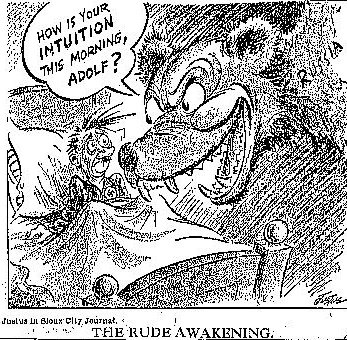
\includegraphics[width=.6\textwidth]{../Figures/Stalingrad.jpg}
      \caption{Ray, S.J. and Star, K.C. ``The Rude Awakening'' [\textit{illegible}] City Journal, 1943}
      \label{fig:1}
    \end{figure}


\end{justifying}
\centering Word Count: 338

\end{mla}

\end{document}

